\documentclass{beamer}
% AnnArbor  Antibes  Bergen  Berkeley  Berlin  Boadilla  CambridgeUS  Copenhagen  Darmstadt  Dresden  Frankfurt  Goettingen  Hannover  Ilmenau  JuanLesPins  Luebeck  Madrid  Malmoe  Marburg  Montpellier  PaloAlto  Pittsburgh  Rochester  Singapore  Szeged  Warsaw  boxes  default 
\mode<presentation>
    {
      \usetheme{Antibes}
      \setbeamercovered{transparent}
    }
    \usepackage[english]{babel}
    \usepackage[latin1]{inputenc}
    \usepackage{times}
    \usepackage[T1]{fontenc}


    \title[A Case Study in SoF] {A Case Study in Stakeholder-oriented Goal-modeling Framework}
          
    \subtitle{}
              
    \author[Author]{Jipeng Wu \and Eryu Ding \and Bin Luo}
                     
     \institute[Universities of Somewhere and Elsewhere] {
                                 Software Institute\\
                                 Nanjing University
     }
                               
\date[ICSESS 2014]
{ICSESS Presentations, 2014}

\subject{Theoretical Computer Science}
\AtBeginSubsection[]
{
  \begin{frame}<beamer>{Outline}
    \tableofcontents[currentsection,currentsubsection]
  \end{frame}
}

%10~12 minutes oral presentation
\begin{document}

\begin{frame}
  \titlepage
\end{frame}

\begin{frame}{Outline}
  \tableofcontents
\end{frame}

\section{Abstract}   
\begin{frame}{}          %[0]
  \begin{itemize}
  \item We present a requirements engineering framework SoF(Stakeholder-oriented goal-modeling Framework) based on RWS goal methods and KAOS modeling methods.  \pause
  \item This framework provides a consistent guide for requirements acquisition, requirements analysis and requirements validation, the three phases of requirements development. \pause
  \item 
    In the phase of requirements acquisition, SoF adopts structured text in nature language to generate a goal model from interview results. It is applied in the development of a management information system called SDMS for a technology department of a software company. \pause
  \end{itemize}
\end{frame}  

\section{Introduction}  
\begin{frame}              %[1]
  \small{
  \begin{itemize}
  \item
    Goal methods now available are usually limited in a certain phase of requirements development and rely on some specific context.  Considering the overall use of goal methods in requirements development, a goal-modeling framework applied throughout different phases of requirements development is necessary.\pause
  \item
    SoF is not limited in a particular abstraction level. It is a method that traces the practical process of requirement acquisition, requirement analysis and requirement validation.\pause
  \item 
    In addition, current goal frameworks are more focused on analysis and technical details of goal modeling of some phase of requirements development. SoF, however, has a different focus more concentrated on how to use goal models to communicate with stakeholders and acquire feedback more agilely. \pause
  \end{itemize}
  }
\end{frame}

\section{Related Work}
\begin{frame}    {KAOS}               %[2]
  \small{
  \begin{itemize} 
  \item The SoF goal-modeling is based on KAOS methods. \pause
    \begin{enumerate}
    \item KAOS provides a formal description of goal model. 
    \item It defines some meta-concepts—goal, action, agent, entity and event, which can be visualized as nodes.
    \item The edges between nodes capture the semantic links between such abstractions.
    \item Two basic link types are defined—AND/OR.\pause
    \end{enumerate}
  \item
    Van Lamsweerde extended the KAOS visualization with the following types of links: Contributes(+), ContributesStrongly(++), Conflicts(-), and ConflictsStrongly(--). Elicitation of goal model is implemented by asking How/Why questions.\pause
  \item
    The deficiency of the practical use of KAOS methods is that it relies on a specific context of requirements development. SoF applies KAOS methods in concrete development process and offers its context.\pause
  \end{itemize}
  }
\end{frame}


\begin{frame}  {RWS}               %[3]
  \footnotesize{
  \begin{itemize}
  \item RWS annotated the goal model with views of stakeholders(1.agree, 2.not agree, 3.add more goals and 4.no position), which facilitates review and validation and finally conforms the goal model to the real world scene.\pause
    \begin{enumerate}
    \item RWS requires that current system should be captured in the form of rich media(e.g., taking photos, recording videos) and the observation results should be linked to goals, in order to elaborate and validate goals in the follow-up work. The observation results are called Real World Scene. \pause
    \item The RWS approach is focused on goal analysis. It uses rich-media scene materials as basis for adding new goals and elaborating goals. The requirements are validated by requirements developers and domain experts. However the scene materials cannot capture full-scale requirements as observation results in requirements development. Additionally, RWS cannot ensure that the decisions made by requirements developers and domain experts correspond to stakeholders' expectations. \pause
    \end{enumerate}
  \end{itemize}
  }
\end{frame}  

\section{Stakeholder-oriented Goal-modeling Framework—SoF}
\subsection{SoF Process}%Section 3.1 Definition of SoF
\begin{frame}   {Introduction}         %[4]
  \small{
    \begin{itemize}
    \item SoF is a framework guiding the acquition of user requirements. \pause
    \item SoF proposed a method ensuring that the goals correspond to stakeholders' interest and their authentic expectation based on RWS: The parent of a goal must have passed the stakeholder validation everytime before the goal is elaborated. \pause
    \item SoF combines requirements acquition, requirements analysis and requirements validation as one atomic activity, which is called \emph{SoF Elaboration Activity}. Each successful \emph{SoF Elaboration Activity} includes the following phases:
      \begin{enumerate}
      \item listening to stakeholders' opions and update structured text document
      \item elaborating goal models and solve conflicts by means of KAOS goal-modeling
      \item and finally convening stakeholder validation interview
      \end{enumerate}
    \end{itemize}
  }
\end{frame}
\begin{frame}  {Introduction}        %[4]
  \begin{itemize}
  \item If a requirements of the future system need $n$ times of elaboration, its \emph{SoF Elaboration Activity} should be conducted at least $n$ times.\pause
  \item Before all the steps of the \emph{SoF Elaboration Activity} of one requirement have been finished, it is not allowed that the \emph{SoF Elaboration Activity} of another requirement is initiated. \pause
  \end{itemize}
\end{frame}

\begin{frame}          %[5]
  \begin{figure}
    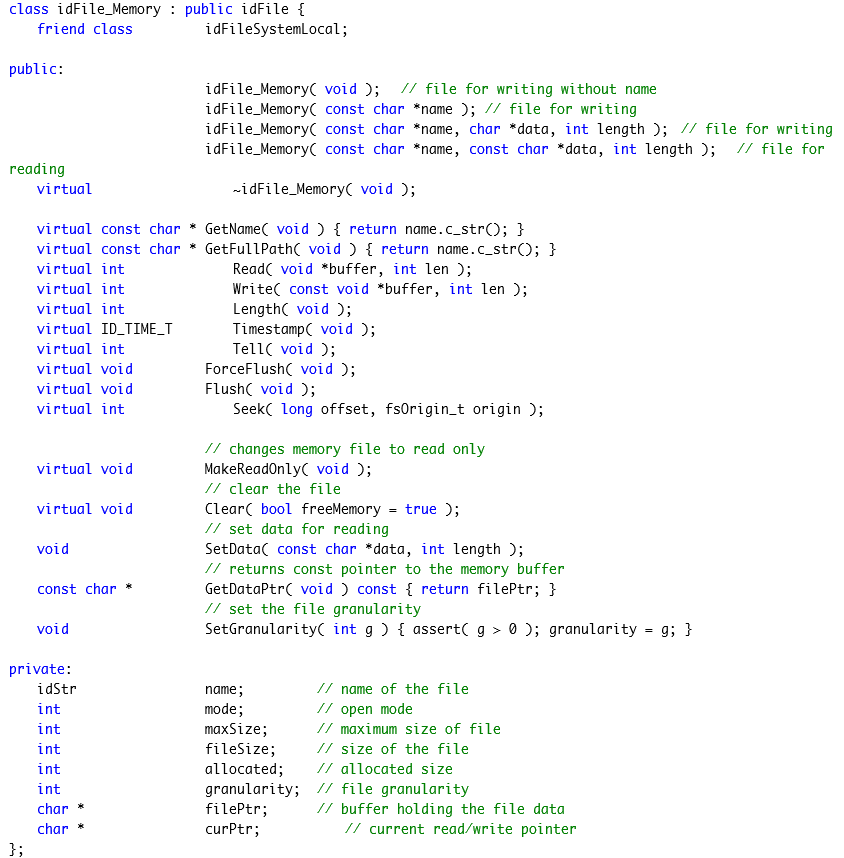
\includegraphics[width=2.4in]{img/2.PNG}
    \caption{Activity Diagram of SoF Process}
  \end{figure}
\end{frame}

\begin{frame}    {As is shown in Fig.1, the 8 detailed steps of SoF is as follows:}        %[6]
  \small{
  \begin{itemize}
  \item %1
    To convene an initial interview, and yield a requirements artefact  $A$. $A$ is a structured text in nature language based on scenario description.\pause
  \item %2
    To analyze $A$ and generate high-level goals: $G_1, G_2, \ldots, G_i, \ldots, G_n (i\in N^+)$. \pause
  \item %3
    To select one leaf-node goal $G_i$.(If this goal $G_i$ is not a high-level goal, the subscript i is a material path, e.g., the first child goal of $G_1$ is $G_{1.1}$). \pause
  \item %4
    To ask How/Why questions about $G_i$ to acquire stakeholders' viewpoints for requirements elaboration.\pause
  \item %5
    To generate $A'$ by adding to $A$ the stakeholders' description of elaborated child goals.\pause
  \end{itemize}
  }
\end{frame}

\begin{frame}     {As is shown in Fig.1, the 8 detailed steps of SoF is as follows:}            %[7]
  \small{
  \begin{itemize}        %$A'\cup A$:  union of the new A and the old one            $B_i$: B sub i
  \item %6                   
    To yield a requirements artefact $B_i$ with information from $A'\cup A$ and knowledge of requirements developers and domain experts. $B_i$ is a SoF annotated goal tree model describing the future system. \pause
  \item %7
    To convene a stakeholder interview to validate the requirements artefact  $B_i$ with the newest version of $A_i$ as a specification of collected stakeholders' viewpoints, and finally yield a requirements artefact  $C_i$. $C_i$ is a SoF annotated tree that has passed the validation. New goals in $C_i$ are marked with $G_{i.j}(j\in N^+)$.\pause
  \item %8
    To rename the temporary $A'$ to $A$ as a formal version. (After this step, the requirements developer should decide whether or not to end the SoF process. To continue SoF process, jump to Step 3 and select another goal.) \pause
  \end{itemize}
  }
\end{frame}

\begin{frame} {Other Features}
  \begin{itemize}
  \item 
    SoF introduces a mechanism against requirements change. It allows stakeholders to send change requests at any time in the SoF process, which is the only legal way to interrupt SoF Elaboration Activities.\pause
  \item 
    The final artefact of SoF is a goal model whose elaboration has passed stakeholder validation. This model is well refined and accepted by stakeholders. It can be a reliable description of user requirements.\pause
  \end{itemize}
\end{frame}


\subsection{Structured Text in Nature Language applied in SoF}
\begin{frame}              %[8]
  \footnotesize{
    \begin{itemize}
    \item SoF adopts a traditional way, conducting a interview, to acquire requirements. It is insufficient to rely only on stakeholders' knowledge and judgment. Thus it is necessary to find a way to specify the description of scenarios of future system from stakeholders and help stakeholders to obtain a consensus.  \pause
    \item SoF uses a structured text in nature language based on scenarios to organize interview results, recording stakeholders' expectations of future system.\pause
    \item 
      The initial interview generates a brief structured specification, describing high-level goals in the form of scenarios. This specification is updated after requirements acquisition phase of each \emph{SoF Elaboration Activity}. Each update is a basis of subsequent goal refinement and goal validation.\pause
    \item 
      The specification is maintained by the requirements development team. They are responsible to update the specification according to change decisions made by stakeholders. Scenarios are used to describe the conceptual model of a future system. The questions posed in stakeholder interviews are based on different scenarios in order to solicit and specify their needs and expectations.\pause
    \end{itemize}
  }
\end{frame}

\subsection{SoF Annotated Goal Tree Model}
\begin{frame}              %[9]
  \footnotesize{
    \begin{itemize}
    \item The goal model adopted by SoF is named after \emph{SoF Annotated Goal Tree Model}. It is based on KAOS and extended by introducing annotations for stakeholder evaluation.\pause
    \item \emph{SoF Annotated Goal Tree Model} is a KAOS goal model which is top-down decomposed. SoF adopts methods from RWS to evaluate requirements with the help of annotated goal models. Only the goals that have passed stakeholder evaluation are allowed to be a basis of elaboration.\pause
    \item 
      The annotations can be used to organize more structured evaluation interviews and actively engage stakeholders in such interviews. More comprehensive engagement among stakeholders allow requirements developers to understand their negotiation, mutual understanding, divergence and consensus of a conceptual future system. After high-level goals determined in an initial interview, the subsequent activities, such as goal elicitation, conflict resolution and requirements evaluation, will be executed based on \emph{SoF Annotated Goal Tree Model}.\pause
    \item More detailed introduction will be presented in the following case study.
    \end{itemize}
  }
\end{frame}

\subsection{Scope of SoF}
\begin{frame}              %[10]
  \begin{itemize}
  \item SoF is not only a method to define goal models. It applies goal models to guide early phase of requirements development.\pause
  \item SoF method is not exclusive. It can be used as supplement of traditional use case model and object-oriented methods.\pause
  \item The primary focus of SoF is the early phase of requirements development. Further refinement to system-level requirements should rely on analysis using other methods, e.g., object-oriented methods.\pause
  \end{itemize}  
\end{frame}


\section{SoF Case Study}
\subsection{Background of SDMS}
\begin{frame}    %[10.5]
  \begin{itemize}
  \item 
    SDMS(Software Departmental Management System) is an information system for the technical department of a software company aimed at improving their efficiency.
  \end{itemize}    
\end{frame}  

\subsection{Structured Specification of Stakeholders’Perspectives}
\begin{frame}     %[11]
  \footnotesize{
    \begin{itemize}
    \item The initial interview poses questions about the background, problem domain, workflow of all possible scenarios of the future system. Requirements developers are responsible for combining information fragments obtained from the interview together to generate a structured specification.\pause
    \item  In the subsequent \emph{SoF Elaboration Activities}, more details will be added in the structured specification in nature language. \emph{SoF Annotated Goal Tree Model} and the structured specification based on scenarios are continuously ameliorated when top-down \emph{SoF Elaboration Activities} are carried out gradually. After SoF process, these requirements artefacts can reach the same level of completeness.\pause
    \item Fig.2 presents a structured description of a scenario of SDMS. It specifies possible events, trigger events of these events and concrete actions of stakeholders in these events in nature languge. Fig.2 does not present a cursory description of high-level goals. It is a specification of a scenario which have passed one \emph{SoF Elaboration Activity} and have been enriched with some details.\pause
    \end{itemize}
  }
\end{frame}

\begin{frame}          %[11.5]
  \begin{figure}
    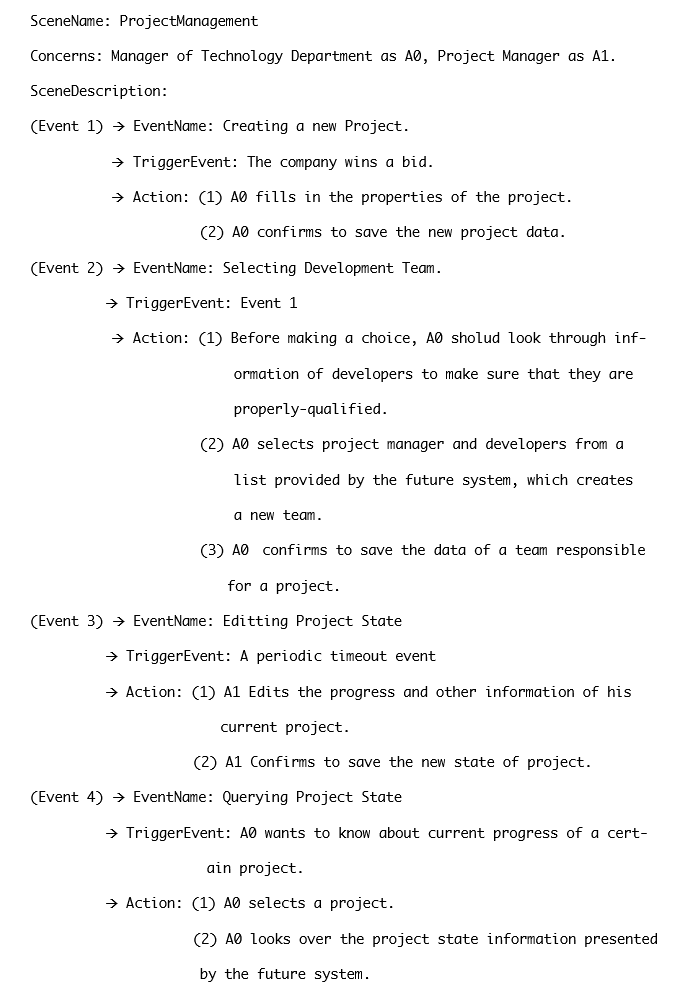
\includegraphics[width=2.4in]{img/3.PNG}
    \caption{Structured Specification of Stakeholders' Perspectives}
  \end{figure}
\end{frame}

\begin{frame}     %[12]
  \footnotesize{
    \begin{itemize}
    \item
      In this example, stakeholders describe the scenario how a technical manager manage projects.
      This scenario includes four events:
      \begin{enumerate}
      \item \emph{create a project}
      \item \emph{select development team}
      \item \emph{edit project info}
      \item \emph{and query project progress}
      \end{enumerate}
    \item 
      Details of these events are specified in the form of triggering events and action description.
      Requirements developers can implement the step of goal elaboration in \emph{SoF Elaboration Activities} based on this specification.
      For example, they can decompose the high-level goal, \emph{improve efficiency of project management}, to several child goals supporting this goal.\pause
    \end{itemize}
  }
\end{frame}
\begin{frame}     %[12]
  \footnotesize{
    \begin{itemize}
    \item 
      The grammar and structure of such structured description can be defined by requirements developers. The main purpose is to organize readable documents from requirements fragments in accordance with their scenarios for the convenience of modification of subsequent work and requirements evaluation.\pause
    \item
      This structured descriptive document does not require rigorously strict grammar.
      It should be informal and simple enough.
      At the highest level of abstraction of requirements, we do not require strict and exact formal statement.
      It is more important to improve the intelligibility of the specification and control the cost of documentation.
      The specification is used only as a basis of evaluation of goal models of the future system.
      However it is not used in any steps of requirements analysis, such as requirements elaboration and solving goal conflicts, which are in the charge of \emph{SoF Annotated Goal Tree Model}.\pause
    \end{itemize}
  }
\end{frame}


\subsection{SoF Annotated Goal Tree Model}
\begin{frame} {Introduction}    %[13]
  \footnotesize{
    \begin{itemize}
    \item \emph{SoF Annotated Goal Tree Model} that has not passed evaluation is a driven model for communication with stakeholders and control of requirements changes. \emph{SoF Annotated Goal Tree Model} that has passed evaluation is a basis of the next \emph{SoF Elaboration Activity}.\pause
    \item We designed a comparatively simpler annotation in the case SDMS because there are no complex stakeholder constituents or serious interest conflicts. The annotation of \emph{SoF Annotated Goal Tree Model} can be modified if more complex evaluation process design is required.\pause
    \item Evaluation phase of \emph{SoF Elaboration Activity} can be further decomposed according to the design of annotations of \emph{SoF Annotated Goal Tree Model}. SDMS adopts two evaluation steps: relevance validation and success validation. \pause
    \end{itemize}
  }
\end{frame}

\begin{frame}{\emph{SoF Annotated Goal Tree Model} adds the following two types of marks:}            %[14]
  \small{
  \begin{itemize}
  \item
    The mark "relevance" is used to record whether a goal has passed relevance validation.
    The evaluation is based on stakeholders perspectives and latest structured specification based on scenarios.
    If the goal is irrelevant to the future system, it is marked with No, otherwise it is marked with Yes.
    Goals cannot enter the next step of success validation until it passes the relevance validation.\pause
  \item
    The mark "agreed" is used to record whether a relevant goal has passed success validation.
    The evaluation is based on stakeholders perspectives on the practical significance, constraints and cost of the evaluated goal. If a it does not agree with stakeholders' expectations, the goal should be still denied.\pause
  \end{itemize}
  }
\end{frame}

\begin{frame} {Goal Elaboration}    %[15]
  \small{
    \begin{itemize}
    \item
      The process of requirements elaboration is consistent with KAOS process. Requirements conflicts should be solved during elaboration processes. In addition, the precondition of elaboration of a goal is that it has passed both steps of evaluation. \pause
    \item
      In practical modeling, all the high-level goals should be completed in one diagram. This paper only presents a elaboration process of one of the high-level goals.\pause
    \end{itemize}
  }
\end{frame}
\begin{frame}  {Goal Elaboration}
  \footnotesize{
    \begin{itemize}
    \item
      \begin{enumerate}
      \item  In Fig.3 we presents a high-level goal $G_1$—"To make technical department manager make better decisions when build project teams".
      \item  By asking Why/How questions we get child goals supporting $G_1$: $G_{1.1}$ and $G_{1.2}$.
        \begin{enumerate}
        \item  $G_{1.1}$ is "To provide better support of information on developers and project managers for techinical department manager".
        \item  $G_{1.2}$ is "To provide a mechanism allowing developers to reply with feedback to the manager's decisions".
        \end{enumerate}
      \item  These two goals were validated as child goals supporting their parent goal in different aspects, and thus successfully passed relevance validation. Stakeholders agreed that these two goals are consistent with their expectations. The goal tree was allowed to be further refined after each goal had passed both validations.\pause
      \end{enumerate}
    \end{itemize}
  }
\end{frame}

\begin{frame}  {Goal Elaboration}
  \begin{figure}
    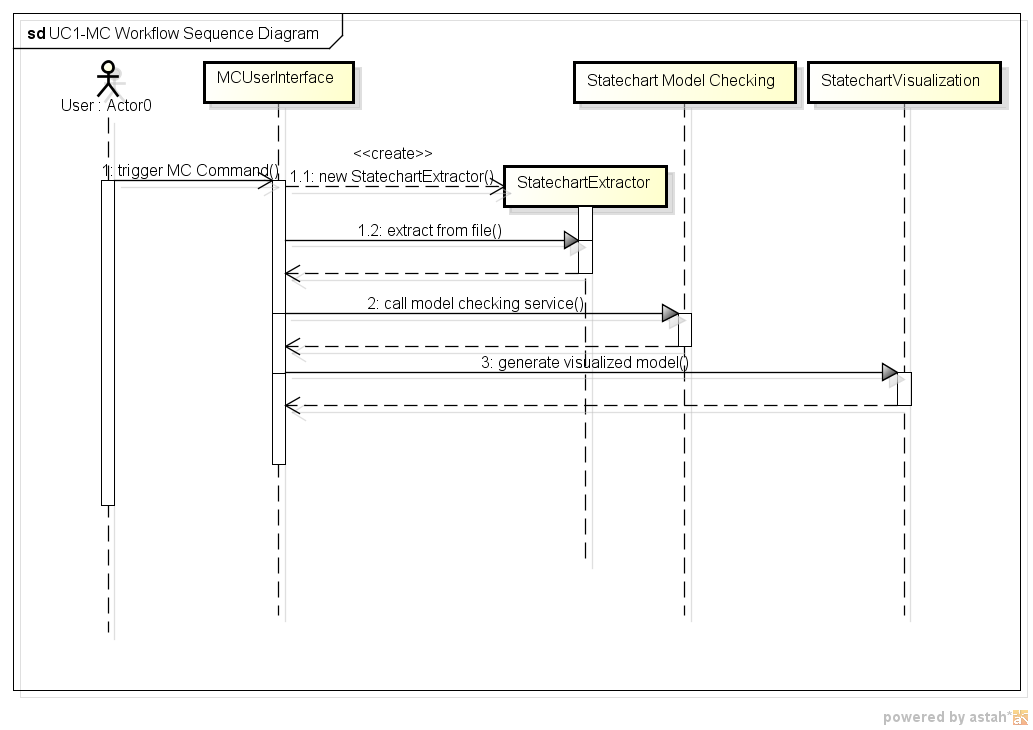
\includegraphics[width=3.4in]{img/4.PNG}
    \caption{SoF Annotated Goal Tree(Validated,Level 1 Elaboration)}
  \end{figure}
\end{frame}

\begin{frame}  {Further Elaboration}   %[16]
  \footnotesize{
    \begin{itemize}
    \item
      In Fig.4, we get a complete \emph{SoF Annotated Goal Tree Model} that has been further elaborated. To emphasize the grammar,  we omit detailed description of each goal in Fig.4 and represent each goal only with its indexed symbol.\pause
    \item
      Here lists the detailed description of each goal that is not mentioned above.
      \begin{enumerate}
      \item $G_{1.1.1}$ is "Project managers input information of developers". 
      \item $G_{1.1.2}$ is "To access information of developers". 
      \item $G_{1.1.3}$ is "Project managers should update information of developers periodically". 
      \item $G_{1.1.1}$、$G_{1.1.2}$、$G_{1.1.3}$ work together to support their parent goal.
      \end{enumerate}
      If any of them fails to pass the evaluation, the whole elaboration plan fails.\pause
    \end{itemize}
  }
\end{frame}
\begin{frame} {Further Elaboration}
  \footnotesize{
    \begin{itemize}
    \item
      \begin{enumerate}
      \item $G_{1.2.1}$ is "To provide an instant messaging platform for technical department managers, project managers and developers".
      \item  $G_{1.2.2}$ is "To publish decisions made by technical department managers and allow developers and project managers to reply asynchronously".
      \item $G_{1.2.1}$ does not conflict any other goal, and facilitates $G_{1.1}$ because the establishment of communication platform contributes positively to technical department managers' knowledge of developers' information. Thus $G_{1.2.1}$ passed both validations.
      \item $G_{1.2.2}$, although had passed the relevance validation, however, failed to pass the success validation because stakeholders believe that asynchronous communication is not practical and efficient enough to ensure the timeliness and richness of feedbacks.      
      \end{enumerate}
    \end{itemize}
  }
\end{frame}

\begin{frame} {Further Elaboration}
  \begin{figure}
    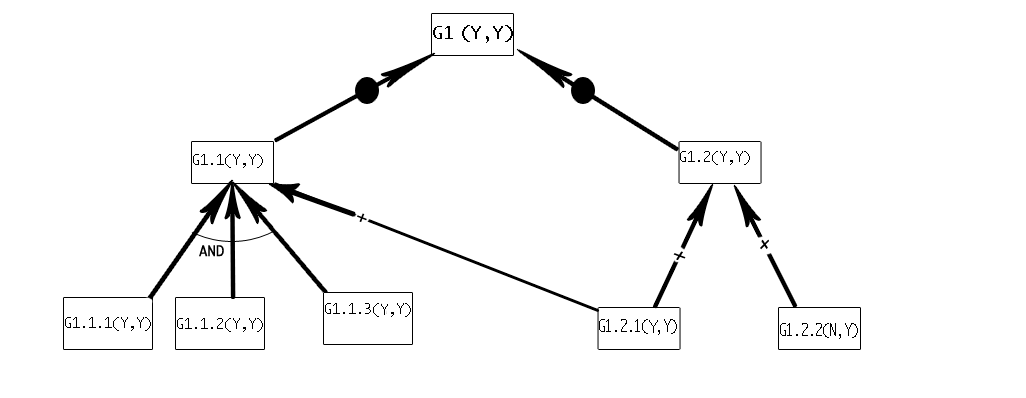
\includegraphics[width=3.4in]{img/5.PNG}
    \caption{SoF Annotated Goal Tree(Validated,Level 2 Elaboration)}
  \end{figure}
\end{frame}    

\section{Discussion}
\begin{frame}{Conclusion:} %[16]
  \small{
  \begin{itemize}
  \item
    SoF can effectively acquire more exact requirements in practice of projects with nondeterminism of requirements. Each step of SoF activities is stakeholder-centered, which ensures that stakeholders' description of future system consists with goal models. With such consistency, SoF provides a reasonable context for KAOS application.\pause
  \item
    \emph{SoF Annotated Goal Tree Model} is an effective tool for not only analysis but also communication. In SDMS practice, structured nature language adopted by SoF is also proved an acceptable method to organize results of interviews, although its effectiveness and its cost control still require further validation from more practical cases.\pause
  \end{itemize}
  }
\end{frame}  

\begin{frame}{Cost Problem:}
  \small{
  \begin{enumerate}
  \item The development cost is relatively higher because recursively executing SoF Elaboration Activities requires considerably frequent communication between and among requirements developers and stakeholders, which will certainly result in unacceptably high cost under some circumstances.\pause
  \item
    One of the most important sources of cost is the collection and management of structured specifications in nature language. We need to find a better way to process raw data from stakeholders.\pause
  \item 
    Another source of cost is the ubiquitous involvement of stakeholders. We should decide whether a project is adaptive in applying SoF methods at the beginning of each project. Some projects with relatively constant and determinate requirements are not supposed to apply SoF methods.\pause
  \end{enumerate}
  }
\end{frame}


\begin{frame}{Unfinished Work:}
  \small{
  \begin{itemize}  
  \item
    SoF process exactly describes each step of early phase of requirements development, but there are still some steps rely on intuition and experience of requirements developers, e.g., how to extract effective high-level goals from the first structured specification in nature language.
  \item 
    Current SoF methods lack a guide to the process of acquisition, analysis and validation of highest-level goals, which requires that requirements developers should make decisions under circumstance of inadequate information. These decisions cannot be reasonably evaluated.
  \item 
    Another topic omitted by SoF is how to use goals to organize scenarios, that is how to link strategic scenarios to tactical scenarios(i.e., high-level goals). \pause
  \end{itemize}
  }
\end{frame}  


\begin{frame}
  \begin{center}
    \Huge{Q \& A}
  \end{center}
\end{frame}  



\end{document}

